\chapter{Casing}

It might seem like the casing is not a very significant part of this project, but the design and function of all kinds of devices' exteriors are crucial. Even the simplest casings often have multiple design stages and variations with different strengths. Since the Tesla coil is intended as a consumer product, the casing plays an essential role in its appearance. However, apart from optics, there are many safety hazards, which the casing has to account for. Most notably is the genuine fire risk, which goes along playing with open plasma.


\section{Concept design}
\label{sec:concept-design}

There are four main parts that are essential to consider while constructing the Tesla coil - the primary coil, the secondary coil, the \glsunset{pcb}\gls{pcb}, and the top electrode. Theoretically, only the placement of the two coils are relevant for its correct operation, but a reasonable practice is to keep everything as close together as possible.

\begin{marginfigure}[1cm]
    \centering
    \includegraphics[width=1.2\textwidth]{kassandra/resources/JerJerWoBistDuKonzept.PNG}
    \caption{Concept design}
    \label{fig:envision}
\end{marginfigure}

As shown in figure \ref{fig:envision}, the secondary coil is perpendicular, and the primary coil is angled at 30° to the horizontal. The primary coil design choices have already been detailed in the previous part at the end of section \ref{sec:designing-the-primary}. The secondary coil has a simple cylindrical form as this is the most straightforward and well-proven design.

The Tesla coil has to provide a breakout point for the arc, which in theory could be any sharp conductive object, even the secondary wire itself. However, due to the high temperatures involved, it would quickly melt away and a separate top electrode is needed. It has to be out of a high temperature resistant material that is also conductive. The placement for the top electrode seems very obvious, but it is not without a reason. As the top electrode is directly connected to the secondary coil, it \emph{becomes} a part of the secondary coil and changes its properties. It is desirable to keep this effect as small as possible by keeping the electrode short and close to the coil. If the breakout point of the electrode is placed further away from the secondary, the behavior of the coils will become less predictable the more distance is between them. So the most practical placement is in the middle and a few centimeters above the secondary coil.

Technically, the \gls{pcb} can be placed anywhere\sidenote{However not too close to the coils to avoid \gls{emi}.} as long as it can be conveniently connected to the coils. However, as a consumer product, the whole device should be as compact and self-contained as possible, which can be achieved by placing the \gls{pcb} right beneath the coils. This way, everything is kept in one place. 

\section{Materials}

Selecting the right materials for every part of the coil plays a crucial role for its correct operation. There are a lot of details and possibilities that have to be considered when designing a Tesla coil. Many factors determine the best working material, most affecting the coils directly and therefore being unsuitable, but others were discarded because of their low availability or costly construction. 

Four criteria have been established of which two, namely the temperature resistance which has to be considered for the top electrode and its surroundings, and the magnetic permeability, which is important around the secondary coil. Unfortunately, due to the limited budget, some materials also turn out as unsuitable because of their price. Optics, the fourth criteria was given the least priority.

\subsection{Metals}
\label{subsec:materials-metals}

Metal is a popular choice for building high-grade casings because of its sturdiness, low price and good machinability. However, metals are rather unsuitable for a Tesla coil, mainly because of their electrical conductivity, which would pose an unnecessary safety risk to the user when touched. On one side, because some internal connection error could in the worst case be lethal, but also because if not properly grounded, static electricity could build up in the casing and shock everyone touching it. Another issue is that metals have a very high permeability, weakening any magnetic field. This would not be a big problem for the \gls{pcb} enclosure but would certainly cause issues when used for the supports of the primary and secondary coil.

\subsection{Woods}

One material that is rarely used for casings, especially for commercial products, is wood, mainly because it is more expensive and harder to work with than metal. Even here, wood is not a good option, mostly because of the anxiety involved in keeping an open plasma flame near a piece of inflammable wood. The same is true for the \gls{pcb} enclosure, because the high voltages present in the circuitry are in the worst case more than capable of creating a spark.

\subsection{Glass}

Glass is an electrical insulator, does not interfere with magnetic fields, has very high-temperature resistance, and has a very polished look. It also comes in various opacities and surface finishes making the casing's appearance very customizable. The big disadvantage tough is its high production costs, which unfortunately also eliminates it as a possibility.

\subsection{Plastics}

\glsunset{pvcp}\glsunset{pmma}\glsunset{pvcu}\glsunset{ptfe}
The only remaining option for the casing's material would be some sort of plastic. The two types of plastic which were available in the workshop, were \gls{pvcp} and \gls{pmma}\sidenote{also commercially known as acrylic glass or plexiglass}. There is also \gls{pvcu}, which is superior to \gls{pvcp} in some aspects, but less available and harder to process. \gls{pvcp} is cheaper and more widely available than \gls{pmma}, however inferior in some other critical regions.

One problem with \gls{pvcp} is its water absorption because due to water's diamagnetic properties, it heats up in an oscillating magnetic field, i.e., it dissipates energy. Its water absorption over 24 hours lies at a maximum of 1\% of its total weight. \gls{pmma}, in comparison, has an absorption factor of at most 0.4\%. On the other hand, \gls{pvcu} has an even more ideal water absorption levels of under 0.1\%. \sidecite{water-absorption} The casing should not be made out of \gls{pvcp} or \gls{pvcu} because of their poor temperature resistance, which start to deform at around 60°C, while \gls{pmma} only starts at about 100°C. \gls{pmma} is not ideal in any way, but due to its easy availability and better properties compared to the other options, it was chosen for the casing. 

The most ideal plastic would be \gls{ptfe}\sidenote{commercially also known as Teflon}, which has a maximum of 0.01\% water absorption, a ten times better than \gls{pvcu}. The temperature resistance is also superior than \gls{pmma} because it can be used at working temperatures up to 280°C\sidecite{blue-bible}. However, \gls{ptfe} was not used, because it has not been taken into consideration until very late projects stages, but will definitively be considered in future builds.

\subsection{Conclusion}

Figure \ref{fig:material-score} summarizes all previously discussed materials by giving them a subjective score from one to ten in the four major categories. The total score shown in the circle is then determined by taking the average points of these categories, and visualizes which material is best suited for the Tesla coil.

\begin{marginfigure}[12mm]
    \centering
    \begin{tabular}{c@{\hskip 1.5mm}p{4cm}}
        {\color{gr70}\faIcon{magnet}} &  Electromagnetic Properties \\
        {\color{gr70}\faIcon{fire}} &  Temperature resistance \\
        {\color{gr70}\faIcon{euro-sign}} &  Machinability and cost \\
        {\color{gr70}\faIcon{eye}} &  Optics
    \end{tabular}
\end{marginfigure}

\begin{figure}[h!]
    \centering
    \begin{tabular}{cc}
      \materialscore{Metal}{4}{1}{8}{6}{3} & \materialscore{Wood}{5}{6}{2}{7}{6} \\
      \materialscore{Glass}{7}{9}{9}{1}{10} & \materialscore{PMMA}{8}{8}{6}{9}{7} \\
      \materialscore{PVC-U}{7}{9}{6}{9}{5} & \materialscore{PTFE}{8}{10}{7}{8}{6} \\
    \end{tabular}
    \caption{Material Score}
    \label{fig:material-score}
\end{figure}



\section{Structure for the Coils}

As mentioned in section \ref{sec:concept-design}, both coils have a fixed position and shape, but to ensure this, the casing has to be built around them. The secondary is easy to support, but the primary has a unique shape that has to be kept in form. 

\subsection{Primary Coil}

The primary coil's holding structure consists of six supports arranged in a hexagonal form. Every support is a sloped plate with an angle of 30°, on top of which the primary coil rests. In order to keep the coil in place, small half-circles have been cut out for every winding. To keep the coil's shape, the slots on each support have to be adjusted to the current radius of the coil.

\begin{figure}[h!]
    \centering
    \includegraphics[width=1\textwidth]{kassandra/resources/endeMeinerHoffnung.png}
    \caption{3D view of the primary supports}
    \label{fig:primary-supports}
\end{figure}

To avoid gluing the supports to the base plate, a bolt was used to keep it in place, as shown in figure \ref{fig:stayer}. This mechanism was mainly designed for testing purposes as it is easier to assemble and disassemble. In a possible future version or commercial release, it would be safer if the supports were glued on. Also, as shown, the supports have a unique design. This was mostly done to make them look elegant and not stand out too much. That makes them lighter, but given that the supports are just a tiny fraction of the Tesla coil's weight, it does not make much of a difference.

\begin{figure}[h!]
    \begin{subfigure}{0.5\textwidth}
        \centering
        \includegraphics[width=\textwidth]{kassandra/resources/endeMeinerHoffnungInSemi2DStayer.PNG}
    \end{subfigure}%
    \begin{subfigure}{0.5\textwidth}
        \centering
        \includegraphics[width=0.7\textwidth]{kassandra/resources/endeMeinerHoffnungIn3DStayer.PNG}
    \end{subfigure}
    \centering
    \caption{Fastening of the supports}
    \label{fig:stayer}
\end{figure}

\subsubsection{Manufacturing}

Small, complex structures like the primary supports are best manufactured with an automated process like 3D printing. This makes it possible to print both the supports and the platform they are mounted on in one part, erasing the need for bolts entirely. Because of the way 3D printing works by drawing multiple layers of fine plastic lines, the final part ends up very inaccurate. This makes it unsuitable for the small half circles on the supports, as they will most likely end up too small for the wire of the primary coil. 

Another way to manufacture the supports would be to laser cut them out of a 5\,mm plastic sheet. This method only allows to construct 2D components, which means that the supports and the platform had to be made separately. One big advantage is its high accuracy, which ensures that the slots for the primary and the bolts fit with only minor post-processing. 

\subsection{Secondary Coil}

The core of the secondary coil was one of the easier parts to design because it essentially just consists of a \(30\,mm\) \gls{pmma} tube with a wall thickness of 3mm and a length of 120\,mm. A few millimeters from the top of the tube, a small hole was drilled to guide the wire to the inside and connect it to the top electrode. The 330 turns of \(0.35\,mm\) wire were wound by hand and then coated with protective and insulating varnish to prevent the wire from loosening and cross-arcing to occur.

\section{Primary Wire Bending}

After the supports for the primary coil have been designed, the coil itself still has to be bent. Simply bending the wire by placing it in the slots one after another is not an option because it takes a considerable amount of force to hold a tensioned \(1.2\,mm\) wire in place\sidenote{This force could be brought up by glue, but that would be very unprofessional}. 
This force is due to the elastic component of the wire's deformation, which tries to bend the wire back to its original shape. 

\subsection{Springback}

To remove this component, the wire has to be overbend by a specific angle and to a specific radius. Those values are determined by the springback factor \(k_s\)\sidecite{blue-bible}, and the desired angle and radius, which remain due to purely plastic deformation. \(k_s\) highly depends on the material and geometry, and usually can be found in large databases.

However, since those are often not freely available\sidenote{Especially not for silver-coated copper wires}, this factor had to be measured by hand. This was done by bending the wire by a specific angle \(\alpha_1\) and measuring the angle \(\alpha_2\) that it sprung back to. Because \(k_s\) is geometry-dependent, this measurement had to be repeated for multiple diameters. \(k_s\) is then defined as the ratio between \(\alpha_2\) and \(\alpha_1\). Figure \ref{fig:springback} shows these calculated values as well as their linear regression fit.

\begin{marginfigure}[-1cm]
    \centering
    \resizebox{0.98\textwidth}{!}{
    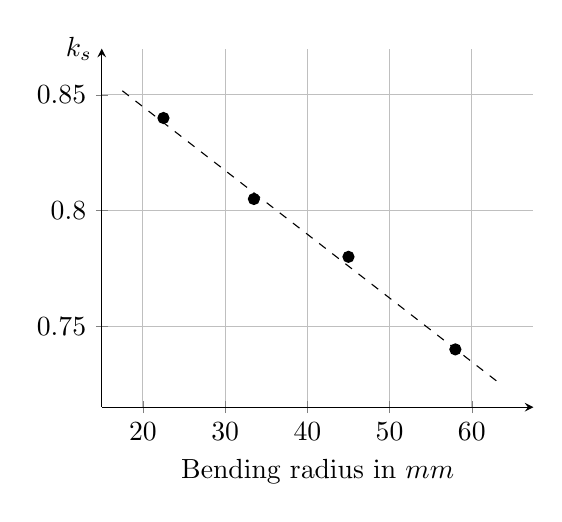
\begin{tikzpicture}
      \begin{axis}[
        xlabel=Bending radius in \(mm\),
        ylabel=\(k_s\),
        y label style={at={(axis description cs:0,1)},rotate=-90},
        grid=major,
        axis lines=left,
        ymin = 0.715,
        ymax = 0.87,
        xmin = 15,
        xmax = 67.5,
        scale = 0.8
        ]
        \addplot[only marks] coordinates{(22.5,0.84)(33.5,0.805)(45,0.78)(58,0.74)};
        \addplot[domain=17.5:63.5, dashed] {-0.002756 *x + 0.9};
      \end{axis}
    \end{tikzpicture}}
    \caption{Springback factor of the copper wire}
    \label{fig:springback}
\end{marginfigure}

In the domain of 25 to 55\,mm, which is the radius of the innermost and outermost winding of the primary coil, the springback factor looks very linear. The equation for the linear regression fit is \(k_s(r_1) = -0.002756 r_1 + 0.9\), where \(r_1\) is the radius, the wire has to be bent to. The necessary bending radius can be calculated as

\begin{equation}
    r_1 = k_S(r_1) \cdot \left(r_2 + r_w\right) - r_w\,,
\end{equation}

where \(r_2\) is the desired constant radius and \(r_w\) is the wire radius. Solving this equation for \(r_1\) gives

\begin{equation}\label{eq:r1-overbending}
    r_1 = \frac{0.9 \cdot \left( r_2 + r_w \right) - r_w}{1 + 0.002756 \cdot \left(r_2 + r_w\right)}\,.
\end{equation}

In the end, the goal is to create an expression which describes the shape the wire has to be bent into. The first important piece of information is the equation for the curve of the secondary coil\sidenote{To be correct, the projection of the curve along its symmetry line}, which can be described as

\begin{equation}\label{eq:r2-spiral}
    r_2 = 25 + \frac{1.5}{\pi} \theta\,.
\end{equation}

Inserting equation \ref{eq:r2-spiral} into equation \ref{eq:r1-overbending}, setting \(r_w\) to \(0.6\,mm\) and simplifying the equation yields that

\begin{equation}
    r_1 = 326.56 - \frac{248622}{\theta + 813.557}\,.
\end{equation}

Figure \ref{fig:spirals} shows \(r_1\) and \(r_2\) side by side for the domain of \([0:20\pi]\).

\begin{figure}[h!]
    \centering
    \resizebox{0.6\textwidth}{!}{
    \begin{tikzpicture}
      \begin{polaraxis}[
        xmin = 270,
        xmax = 450,
        ymax = 60,
        xticklabels = {,,},
        yticklabels = {,,},
        ]
        \addplot[domain=0:20*pi, samples=500, color=black!60, data cs=polarrad] { 25 + 0.4775 * x };
      \end{polaraxis}
      \begin{polaraxis}[
        xmin = 90,
        xmax = 270,
        ymax = 60,
        xshift = -3.43cm,
        xticklabels = {,,},
        ]
        \addplot[domain=0:20*pi, samples=500, color=black!60, data cs=polarrad] { 326.56 - 248622 / (x+813.557) };   
    \end{polaraxis}
\end{tikzpicture}}
    \caption{AAA}
    \label{fig:spirals}
\end{figure}

Even though it looks like \(r_1\) has a uniform inclination, the distance between each turn actually falls with an increasing radius. This is because the bigger the bending radius, the more it must be overbent. In this case, the distance between the two innermost turns is about \(2.578\,mm\), while the distance between the two outermost turns is only \(2.262\,mm\).

During the transformation from \(r_1\) to \(r_2\), the wire not only increases its diameter but also decreases its number of turns. This is because the total length of the wire has to stay the same. The overbending angle \(\alpha_1\), which directly relates to the number of turns, is simply the remaining angle \(\alpha_2\) divided by \(k_s\). However, \(k_s\) is a function of \(r_1\), which in turn is a function on \(\alpha_1\), which is a function of \(\alpha_2\). Since this does not only sound impractical, another approach was taken.

% sounds weird
The domain of \(r_1\) has to be chosen so that its length is the same as the length of \(r_1\) in the domain \([0:20\pi]\). To calculate the length of the curves, a WolframAlpha widget\sidenote{an URL to which can be found in QR code \newqrcode{https://www.wolframalpha.com/widgets/view.jsp?id=c26cbb9457ff75f58f479364ddb79cd1}{Arc Length in Polar Coordinates}} has been used. In the domain \([0:20\pi]\), the length of the curve \(r_2\) turns out to be \(2.51\,m\) while \(r_1\) is with just above \(2\,m\) a little too short. By using the trial-and-error method, it has been found that \(r_1\) needs to have \(11.77\) turns to achieve the desired length.

However, one remaining problem is that \(r_2\) is only the projection of the actual primary coil. A conic spiral is longer than its flat projection and also needs to be bent, which introduces additional springback. However, the average inclination of the wire is with \(1.7\,mm\) per turn, only about \(0.0002\) degrees, which is negligible.

\subsection{Bending Device}

Since bending a wire according to a specific curve equation just by looking at it is rather hard, a bending device was designed. It is just a cone with a spiral-shaped grooving, where the wire can be pressed into. After taking it out again, it bends on the correct form of the primary coil. The grooving was made slightly wider than the wire’s diameter to ensure that the wire does not get stuck.

The trickiest part was drawing the path for the grooving in Autodesk Inventor. First, a 2D spiral was drawn by adding a polar equation curve for \(r_1\), which was then projected onto a conical plane as shown in figure \ref{fig:spirae}. Designing the rest of the bending device was relatively straightforward, and figure \ref{fig:biegbieg} shows a sliced view of the final part.

\begin{marginfigure}[-3cm]
    \centering
    \includegraphics[width=0.9\textwidth]{kassandra/resources/JerJerWoBistDuSpirae.PNG}
    \caption{Projected Curve for the Bending Device}
    \label{fig:spirae}
\end{marginfigure}

\begin{figure}[h!]
    \centering
    \includegraphics[width=0.7\textwidth]{kassandra/resources/JerJerWoBistDuBiegeBieg.PNG}
    \caption{Bending Device}
    \label{fig:biegbieg}
\end{figure}

Given this device's peculiar shape, which has to be very accurate\sidenote{when it comes to shape}, the best way to manufacture would be 3D printing. Even though the grooving was made bigger, the wire was still hard to press into the bending device because of how a 3D printer work. In the end, the bent wire of the primary still had to be glued to the supports so it would not fall off. 

\section{Top Electrode}

The top electrode needs to be made out of a temperature resistant, conductive material. It should already be available as thin rod, because turning would not be an option for such a small diameter. Welding electrodes fit this criteria, because they are a few millimeters thick and consist of a tungsten alloy with a melting point of around \texttt{insert correct value here}. By using a bench grinder, one side of the electrode could easily be whetted to a pointy spike.

The holder that keeps the electrode at the top of the coil is made out of two elements. As seen in figure \ref{fig:top-electrode}, the first one is two copper pieces that are kept together with a thread, and lock the wire tight in between. There are two notches on each one to be able to fasten and open them with a flat wrench. To mount the tungsten electrode, a press fit was drilled into the top surface of the copper piece. The second part is a \gls{pmma} piece in which the first part is mounted. It has a slit on one side to be able to take out the copper piece without releasing the wire first.

\begin{marginfigure}[-8cm]
    \centering
    \includegraphics[width=0.7\textwidth]{kassandra/resources/endeMeinerHoffnungFürBlitz.PNG}
    \caption{Mounting of the top electrode}
    \label{fig:top-electrode}
\end{marginfigure}

\subsection{It's not a Bug, it's a Feature}

Because the Tesla coil driver was very under-dimensioned, the plasma flame forming on the top electrode was very small and often had to be ignited and stabilized by another conductor held close to it. This was realized by placing a second, ancillary electrode over to the main electrode. This electrode is held by a canopy-like structure, which rests on three \gls{pmma} rods. It was press fitted into a flat copper cylinder, which was loosely screwed into the cap. This way, its height and the gap between the two electrodes can be changed by turning the ancillary electrode.

\begin{marginfigure}[-3cm]
    \centering
    \includegraphics[width=\textwidth]{kassandra/resources/mirGehtsSuperDanke.png}
    \caption{Mounting of the ancillary electrode}
    \label{fig:ancillary-electrode}
\end{marginfigure}

To further examine the effect of the cap's material and shape, three different versions have been produced. One out of \gls{pmma} and two out of Aluminium, one of which is as smooth as possible and one as pointy as possible.

\begin{figure}[h!]
    \centering
    \label{fig:caps}
    \begin{subfigure}[b]{0.4\textwidth}
        \centering
        \includegraphics[width=0.9\textwidth]{kassandra/resources/mirGehtsSuperDankeSmooth.png}
    \end{subfigure}
    \hfill
    \begin{subfigure}[b]{0.4\textwidth}
        \centering
        \includegraphics[width=0.9\textwidth]{kassandra/resources/mirGehtsSuperDankeEdgy.png}
    \end{subfigure}
    \caption{Smooth and Pointy Cap}
\end{figure}

While in section \ref{subsec:materials-metals}, it was explained that metals pose a safety hazard, this is not entirely true for the secondary side of the Tesla coil. Despite the high voltages present at the top electrode, it is relatively safe to touch. This is because the secondary coil cannot provide enough current and power to cause any physical damage, except the usual burned skin due to the flame's heat.

\section{PCB Enclosure}

The general placement of the \gls{pcb}, being right beneath the coils, was already addressed in section \ref{sec:concept-design}. The platform where the secondary coil and the supports for the primary coil are mounted was already designed and chosen to be hexagon-shaped, mainly because it works the best with the six supports. Again, the prototype has the platform resting on top of six pillars to keep everything as modular as possible. The prototype also has only the most essential features and only consists of a framework, this also makes it easier to access the inside of the \gls{pcb} enclosure. The final design would be completely closed off, and the platform would be glued on as like the primary coil’s supports.

\begin{figure}[h!]
    \centering
    \includegraphics[width=0.9\textwidth]{kassandra/resources/JerJerWoBistDu.PNG}
    \caption{PCB Enclosure}
    \label{fig:bottom-bau}
\end{figure}

\subsection{PCB}

The hexagonal \gls{pcb} was placed in the center of the enclosure right under the secondary, mostly to balance the design. To ensure that the circuit can also give off heat on the bottom side, it cannot be mounted directly onto the enclosure and therefore has to be raised by a few millimeters. This is done by six steps onto which the \gls{pcb} is screwed. 

\begin{marginfigure}[-3cm]
    \centering
    \includegraphics[width=0.7\textwidth]{kassandra/resources/JerJerWoBistDuStufe.PNG}
    \caption{PCB Holder}
    \label{fig:bottom_stufe}
\end{marginfigure}
    
